\section{Capítulo 1 -- APIs e Web Services}

Quando você abre o aplicativo do banco e vê o seu saldo, quando um site de compras calcula o frete a partir do CEP ou quando um sistema emite uma nota fiscal eletrônica, há sempre dois programas conversando: um que pede uma informação e outro que a entrega. Essa conversa acontece por meio de uma \textbf{API}. Neste capítulo você vai entender o que é uma API, como funciona o protocolo HTTP, que transporta essas conversas na web, e quais são os principais estilos de serviço web: SOAP, REST e GraphQL. No final, vai consultar uma API pública de verdade e conhecer o projeto que será construído ao longo da apostila.

\subsection{1.1 O que é uma API}

\textbf{API} é a sigla de \textit{Application Programming Interface}, ou interface de programação de aplicações. É um conjunto de regras que define como um programa pode pedir algo a outro: quais pedidos existem, que dados cada pedido precisa receber e o que vem de volta.

Uma comparação comum é a do restaurante. O cliente não entra na cozinha: ele consulta o cardápio e faz o pedido ao garçom, que leva o pedido à cozinha e traz o prato. O cardápio é o \textbf{contrato} da API (o que pode ser pedido), o garçom é a API, e a cozinha é o sistema que faz o trabalho. O cliente não precisa saber como a cozinha funciona, e a cozinha pode mudar de fogão sem que o cliente perceba, desde que o cardápio continue o mesmo.

Esse é o grande valor de uma API: ela \textbf{separa quem usa de quem implementa}. Um mesmo servidor pode atender, ao mesmo tempo, o site, o aplicativo de celular e o sistema de um parceiro, todos usando o mesmo contrato.

O termo API é amplo. As funções de uma biblioteca, como o \texttt{readFile} do Node.js, também formam uma API. Nesta apostila, porém, o foco são as \textbf{APIs web}: aquelas acessadas pela rede, usando o protocolo HTTP. Quando essas APIs são oferecidas por um sistema para ser usadas por outros sistemas, também são chamadas de \textbf{serviços web} (\textit{web services}).

\subsection{1.2 Cliente, servidor e o protocolo HTTP}

Toda conversa com uma API web segue o modelo \textbf{cliente-servidor}: o \textbf{cliente} envia uma \textbf{requisição} (\textit{request}) e o \textbf{servidor} devolve uma \textbf{resposta} (\textit{response}). O cliente pode ser um navegador, um aplicativo de celular ou outro servidor. As regras dessa troca são as do \textbf{HTTP} (\textit{HyperText Transfer Protocol}), o mesmo protocolo que o navegador usa para carregar páginas.

\begin{center}
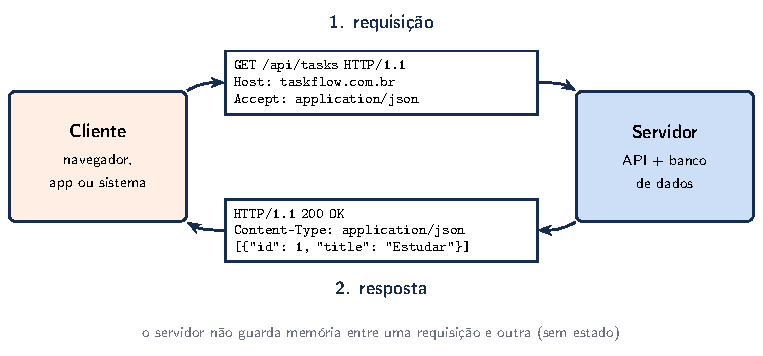
\includegraphics[width=0.95\linewidth,keepaspectratio]{imagens/capitulo-01_requisicao.pdf}
\end{center}

Uma requisição HTTP tem quatro partes:

\begin{itemize}
  \item o \textbf{método}, que diz o que o cliente quer fazer: \texttt{GET} para buscar, \texttt{POST} para criar, \texttt{PUT} e \texttt{PATCH} para alterar, \texttt{DELETE} para excluir;
  \item a \textbf{URL}, que diz em que recurso a ação será feita, como \texttt{/api/tasks};
  \item os \textbf{cabeçalhos} (\textit{headers}), pares nome e valor com informações extras, como o formato aceito na resposta;
  \item o \textbf{corpo} (\textit{body}), opcional, com os dados enviados, por exemplo os campos de uma tarefa nova.
\end{itemize}

A resposta tem três: o \textbf{código de status}, um número que resume o resultado (\texttt{200} deu certo, \texttt{404} não encontrado, \texttt{500} erro no servidor), os \textbf{cabeçalhos} e o \textbf{corpo}, com os dados pedidos. Por baixo de tudo, requisição e resposta são apenas texto. Veja como fica a criação de uma tarefa:

\begin{codigo}
\begin{Verbatim}[breaklines=true, breaksymbolleft={}, fontsize=\footnotesize]
POST /api/tasks HTTP/1.1
Host: taskflow.com.br
Content-Type: application/json

{"title": "Estudar HTTP", "priority": "HIGH"}
\end{Verbatim}
\end{codigo}

\begin{codigo}
\begin{Verbatim}[breaklines=true, breaksymbolleft={}, fontsize=\footnotesize]
HTTP/1.1 201 Created
Content-Type: application/json
Location: /api/tasks/42

{"id": 42, "title": "Estudar HTTP", "priority": "HIGH"}
\end{Verbatim}
\end{codigo}

A linha em branco separa os cabeçalhos do corpo. O cabeçalho \texttt{Content-Type} informa o formato do corpo; aqui, \texttt{application/json}. O status \texttt{201 Created} indica que um recurso novo foi criado, e o cabeçalho \texttt{Location} diz onde ele pode ser encontrado. Os métodos e os códigos de status são estudados em detalhe nos Capítulos 2 e 8.

Uma característica essencial do HTTP é ser \textbf{sem estado} (\textit{stateless}): cada requisição é independente, e o servidor não se lembra das anteriores. Se o servidor precisa saber quem está pedindo, a própria requisição tem de trazer essa informação, normalmente um \textbf{token} em um cabeçalho. É assim que funciona o login em APIs, assunto do Capítulo 9.

\subsection{1.3 A anatomia de uma URL}

A URL (\textit{Uniform Resource Locator}) identifica onde está o recurso. Cada parte tem uma função:

\begin{codigo}
\begin{Verbatim}[breaklines=true, breaksymbolleft={}, fontsize=\footnotesize]
https://api.taskflow.com.br:443/v1/tasks?status=DONE&page=2
\end{Verbatim}
\end{codigo}

\begin{center}
\begin{tabular}{@{}P{0.27\linewidth}P{0.3\linewidth}P{0.33\linewidth}@{}}
\toprule
\rowcolor{headergray}
\tblheader{Parte} & \tblheader{Exemplo} & \tblheader{Função} \\
\midrule
protocolo & \texttt{https} & como a conversa acontece; o \texttt{s} indica conexão criptografada \\
\rowcolor{rowgray} domínio & \texttt{api.taskflow.com.br} & o nome do servidor \\
porta & \texttt{443} & a ``porta de entrada''; 443 é o padrão do HTTPS e costuma ser omitida \\
\rowcolor{rowgray} caminho & \texttt{/v1/tasks} & o recurso dentro do servidor \\
\textit{query string} & \texttt{?status=DONE\&page=2} & parâmetros extras, como filtros e paginação, em pares nome=valor separados por \texttt{\&} \\
\bottomrule
\end{tabular}
\end{center}

Na \textit{query string}, espaços e acentos não podem aparecer como são: eles são codificados, e ``São Paulo'' vira \texttt{S\%C3\%A3o\%20Paulo}. O \texttt{fetch} e as bibliotecas de HTTP cuidam disso com \texttt{encodeURIComponent} ou com a classe \texttt{URLSearchParams}.

\subsection{1.4 Serviços web com SOAP}

Os primeiros serviços web populares, no início dos anos 2000, usavam o \textbf{SOAP} (\textit{Simple Object Access Protocol}), um protocolo padronizado pelo W3C. No SOAP, toda mensagem é um documento \textbf{XML} com uma estrutura fixa, o \textbf{envelope}, e o serviço é descrito em um arquivo \textbf{WSDL} (\textit{Web Services Description Language}), também em XML, que lista as operações, os parâmetros e os tipos de cada uma. A partir do WSDL, ferramentas geram automaticamente o código do cliente.

\begin{codigo}
\begin{Verbatim}[breaklines=true, breaksymbolleft={}, fontsize=\footnotesize]
<soap:Envelope
    xmlns:soap="http://www.w3.org/2003/05/soap-envelope"
    xmlns:t="http://taskflow.com.br/ws">
  <soap:Header/>
  <soap:Body>
    <t:BuscarTarefa>
      <t:id>42</t:id>
    </t:BuscarTarefa>
  </soap:Body>
</soap:Envelope>
\end{Verbatim}
\end{codigo}

Repare que a operação, \texttt{BuscarTarefa}, aparece dentro da mensagem. No SOAP, todas as chamadas costumam ir para uma mesma URL, quase sempre com o método \texttt{POST}, e é o conteúdo do envelope que diz o que fazer. O padrão também define como devolver erros (o elemento \texttt{Fault}) e tem extensões para segurança e transações, como o WS-Security.

O SOAP é verboso e rígido, mas essa rigidez é justamente o que alguns sistemas querem: um contrato formal, validado automaticamente. Por isso ele continua presente em bancos, seguradoras e em sistemas de governo. No Brasil, a emissão da Nota Fiscal Eletrônica (NF-e) é feita por serviços web SOAP das secretarias da Fazenda.

\subsection{1.5 APIs REST}

O \textbf{REST} (\textit{Representational State Transfer}) não é um protocolo, e sim um \textbf{estilo de arquitetura}, descrito por Roy Fielding em sua tese de doutorado, em 2000. A ideia central é organizar a API em torno de \textbf{recursos}, as ``coisas'' do sistema (tarefas, usuários, pedidos), cada um identificado por uma URL, e usar os \textbf{métodos do próprio HTTP} para dizer o que fazer com eles:

\begin{codigo}
\begin{Verbatim}[breaklines=true, breaksymbolleft={}, fontsize=\footnotesize]
GET    /api/tasks       lista as tarefas
POST   /api/tasks       cria uma tarefa
GET    /api/tasks/42    busca a tarefa 42
PATCH  /api/tasks/42    altera parte da tarefa 42
DELETE /api/tasks/42    exclui a tarefa 42
\end{Verbatim}
\end{codigo}

O servidor devolve uma \textbf{representação} do recurso, hoje quase sempre em \textbf{JSON}, um formato de texto leve e fácil de ler tanto por pessoas quanto por programas:

\begin{codigo}
\begin{Verbatim}[breaklines=true, breaksymbolleft={}, fontsize=\footnotesize]
{
  "id": 42,
  "title": "Estudar HTTP",
  "status": "PENDING",
  "priority": "HIGH",
  "dueDate": "2026-11-20"
}
\end{Verbatim}
\end{codigo}

Compare com o SOAP: em vez de uma operação \texttt{BuscarTarefa} escrita dentro de um envelope, o REST usa \texttt{GET} na URL da tarefa. As regras do estilo, como a ausência de estado e o uso de URLs para identificar recursos, são o tema do Capítulo 2. Por ser simples, usar o HTTP como ele foi pensado e funcionar bem com JavaScript, o REST se tornou o estilo dominante nas APIs web, e é o estilo usado nesta apostila.

\subsection{1.6 GraphQL}

O \textbf{GraphQL} foi criado pelo Facebook em 2012 e aberto ao público em 2015. Ele é uma \textbf{linguagem de consulta} para APIs: em vez de várias URLs, há um único endereço, normalmente \texttt{/graphql}, e o cliente envia uma consulta dizendo exatamente quais campos quer receber.

\begin{codigo}
\begin{Verbatim}[breaklines=true, breaksymbolleft={}, fontsize=\footnotesize]
query {
  usuario(id: 7) {
    nome
    tarefas(status: PENDING) {
      title
      dueDate
    }
  }
}
\end{Verbatim}
\end{codigo}

\begin{codigo}
\begin{Verbatim}[breaklines=true, breaksymbolleft={}, fontsize=\footnotesize]
{
  "data": {
    "usuario": {
      "nome": "Ana",
      "tarefas": [
        { "title": "Estudar HTTP", "dueDate": "2026-11-20" }
      ]
    }
  }
}
\end{Verbatim}
\end{codigo}

A resposta tem o mesmo formato da consulta. Isso resolve dois problemas comuns do REST: receber campos demais, que o cliente não vai usar (\textit{over-fetching}), e precisar de várias requisições para montar uma tela, como uma para o usuário e outra para as tarefas dele (\textit{under-fetching}). Em troca, o servidor fica mais complexo, e recursos simples do HTTP, como o \textit{cache} por URL, deixam de funcionar sozinhos. O GraphQL brilha em aplicações com telas muito variadas, como redes sociais; para a maioria das APIs, o REST continua mais simples.

\subsection{1.7 Outros estilos de comunicação}

Três outras formas de comunicação aparecem com frequência ao lado das APIs:

\begin{itemize}
  \item \textbf{gRPC}: criado pelo Google, usa o HTTP/2 e um formato binário, o \textit{Protocol Buffers}, muito mais compacto que o JSON. É comum na comunicação entre servidores de uma mesma empresa, em que o desempenho importa mais que a facilidade de leitura.
  \item \textbf{WebSocket}: abre uma conexão que fica aberta, e o servidor pode enviar dados ao cliente a qualquer momento, sem esperar uma requisição. É a base de chats, placares ao vivo e notificações em tempo real.
  \item \textbf{Webhook}: é o caminho inverso de uma API. Em vez de o seu sistema perguntar de tempos em tempos ``o pagamento foi aprovado?'', o serviço de pagamento faz uma requisição \texttt{POST} para uma URL do seu sistema assim que o pagamento é aprovado.
\end{itemize}

\subsection{1.8 Comparando SOAP, REST e GraphQL}

\begin{center}
\begin{tabular}{@{}P{0.2\linewidth}P{0.23\linewidth}P{0.23\linewidth}P{0.23\linewidth}@{}}
\toprule
\rowcolor{headergray}
\tblheader{} & \tblheader{SOAP} & \tblheader{REST} & \tblheader{GraphQL} \\
\midrule
o que é & protocolo & estilo de arquitetura & linguagem de consulta \\
\rowcolor{rowgray} formato & XML (envelope) & qualquer um; quase sempre JSON & JSON \\
endereços & uma URL por serviço & uma URL por recurso & uma URL só \\
\rowcolor{rowgray} operação indicada & no envelope & pelo método HTTP & na consulta \\
contrato & WSDL, obrigatório & opcional (OpenAPI, Capítulo 10) & esquema, obrigatório \\
\rowcolor{rowgray} uso típico & bancos, governo, sistemas legados & APIs públicas e a maioria dos sistemas web & telas com dados muito variados \\
\bottomrule
\end{tabular}
\end{center}

Nenhum estilo é melhor em tudo. A escolha depende de quem vai usar a API, do tipo de dado e das exigências do sistema. Um mesmo produto pode, inclusive, usar mais de um: REST para o aplicativo, SOAP para falar com o sistema fiscal e WebSocket para as notificações.

\subsection{1.9 Consultando uma API pública}

A melhor forma de entender uma API é usar uma. O \textbf{ViaCEP} é um serviço gratuito que devolve o endereço de um CEP e não exige cadastro. Como a consulta usa o método \texttt{GET}, basta colar a URL no navegador:

\begin{codigo}
\begin{Verbatim}[breaklines=true, breaksymbolleft={}, fontsize=\footnotesize]
https://viacep.com.br/ws/01001000/json/
\end{Verbatim}
\end{codigo}

Pelo terminal, a ferramenta \texttt{curl} faz a mesma requisição e mostra a resposta. Ela já vem instalada no Windows 10 e 11, no macOS e no Linux; no PowerShell, digite \texttt{curl.exe}. A opção \texttt{-i} mostra também a linha de status e os cabeçalhos:

\begin{codigo}
\begin{Verbatim}[breaklines=true, breaksymbolleft={}, fontsize=\footnotesize]
$ curl -i https://viacep.com.br/ws/01001000/json/
HTTP/1.1 200 OK
Content-Type: application/json; charset=utf-8

{
  "cep": "01001-000",
  "logradouro": "Praça da Sé",
  "complemento": "lado ímpar",
  "bairro": "Sé",
  "localidade": "São Paulo",
  "uf": "SP",
  "ddd": "11"
}
\end{Verbatim}
\end{codigo}

A resposta real tem mais campos e cabeçalhos; aqui aparecem só os principais. Em um programa, a requisição é feita com o \texttt{fetch}, que existe no navegador e, desde a versão 18, também no Node.js:

\begin{codigo}
\begin{Verbatim}[breaklines=true, breaksymbolleft={}, fontsize=\footnotesize]
// cep.mjs  -- rode com: node cep.mjs
const cep = "01001000";
const url = `https://viacep.com.br/ws/${cep}/json/`;

const resposta = await fetch(url);
console.log(resposta.status);     // 200

const endereco = await resposta.json();
console.log(`${endereco.logradouro}, ${endereco.localidade}`);
// Praça da Sé, São Paulo
\end{Verbatim}
\end{codigo}

O \texttt{fetch} devolve uma \textit{Promise} com a resposta; \texttt{resposta.status} é o código de status, e \texttt{resposta.json()} lê o corpo e o converte em um objeto JavaScript. Troque \texttt{json} por \texttt{xml} no fim da URL e o mesmo serviço responde em XML, assunto do Capítulo 5.

Experimente também um CEP que não existe, como \texttt{99999999}. O ViaCEP responde com status \texttt{200} e o corpo \texttt{\{"erro": "true"\}}. É uma escolha de projeto discutível: o Capítulo 8 mostra por que, em uma API REST, o mais adequado seria o status \texttt{404}.

\subsection{1.10 O projeto da apostila: a API do TaskFlow}

Ao longo da apostila, você vai construir a API do \textbf{TaskFlow}, um gerenciador de tarefas em que cada pessoa cria uma conta e organiza as próprias tarefas. A cada capítulo, a API ganha uma parte nova, até ser publicada na internet com domínio próprio. As ferramentas são as mesmas usadas por empresas no dia a dia:

\begin{itemize}
  \item \textbf{Next.js} com \textbf{TypeScript}, para criar as rotas da API (Capítulos 3 e 4);
  \item \textbf{PostgreSQL} na nuvem, com o NeonDB, e o \textbf{Prisma} para acessar o banco (Capítulos 3 e 7);
  \item \textbf{Zod}, para validar os dados recebidos (Capítulo 6);
  \item \textbf{JWT}, para a autenticação (Capítulo 9);
  \item \textbf{Vitest}, para os testes automatizados (Capítulo 11);
  \item \textbf{Vercel}, para a publicação (Capítulo 12).
\end{itemize}

Ao final, a API terá estes \textit{endpoints}, ou seja, as combinações de método e URL que ela atende:

\begin{center}
\begin{tabular}{@{}P{0.1\linewidth}P{0.36\linewidth}P{0.44\linewidth}@{}}
\toprule
\rowcolor{headergray}
\tblheader{Método} & \tblheader{URL} & \tblheader{O que faz} \\
\midrule
\texttt{POST} & \texttt{/api/auth/register} & cria uma conta \\
\rowcolor{rowgray} \texttt{POST} & \texttt{/api/auth/login} & entra e recebe um token \\
\texttt{GET} & \texttt{/api/tasks} & lista as tarefas de quem está logado, com filtros \\
\rowcolor{rowgray} \texttt{POST} & \texttt{/api/tasks} & cria uma tarefa \\
\texttt{GET} & \texttt{/api/tasks/:id} & busca uma tarefa \\
\rowcolor{rowgray} \texttt{PATCH} & \texttt{/api/tasks/:id} & altera uma tarefa \\
\texttt{DELETE} & \texttt{/api/tasks/:id} & exclui uma tarefa \\
\bottomrule
\end{tabular}
\end{center}

O \texttt{:id} indica uma parte variável da URL: \texttt{/api/tasks/42} é a tarefa 42. Para acompanhar, você vai precisar do Node.js (versão 20 ou mais nova), do VS Code e de uma conta gratuita no GitHub, que também serve para entrar no NeonDB e na Vercel.

\subsection{Erros Comuns}

\begin{itemize}
  \item \textbf{Achar que API é sinônimo de REST.} REST é um estilo; SOAP, GraphQL e gRPC também são formas de construir APIs.
  \item \textbf{Achar que o servidor ``lembra'' do cliente.} O HTTP é sem estado: cada requisição precisa trazer tudo o que o servidor precisa saber, inclusive quem está pedindo.
  \item \textbf{Confundir a URL com o \textit{endpoint}.} O mesmo caminho, \texttt{/api/tasks}, é um \textit{endpoint} com \texttt{GET} (listar) e outro com \texttt{POST} (criar).
  \item \textbf{Esquecer o \texttt{await} no \texttt{fetch}.} Sem ele, a variável guarda uma \textit{Promise}, e não a resposta. O mesmo vale para \texttt{resposta.json()}.
  \item \textbf{Confiar apenas no status.} Algumas APIs, como o ViaCEP com um CEP inexistente, respondem \texttt{200} e indicam o erro no corpo. Leia a documentação de cada API.
  \item \textbf{Colocar acentos e espaços direto na \textit{query string}.} Use \texttt{encodeURIComponent} ou \texttt{URLSearchParams} para montar os parâmetros.
\end{itemize}
